\chapter{Cholesky transformation results}\label{app:Chol}
In this Appenndix results of Cholesky decomposition for partially correlated uncertainties (see Sec.~\ref{sec:partCor}) are presented. The resulting uncorrelated systematic sources are shown in Fig.~\ref{fig:AppA} in source vs the analysis plane. The content of the cell corresponds to the value of $\delta C/C (\%)$.  The resulted systematic uncertainties are included in averaging process and PDF profiling.

\begin{figure}[!h]
\begin{minipage}[h]{0.39\linewidth}
\center{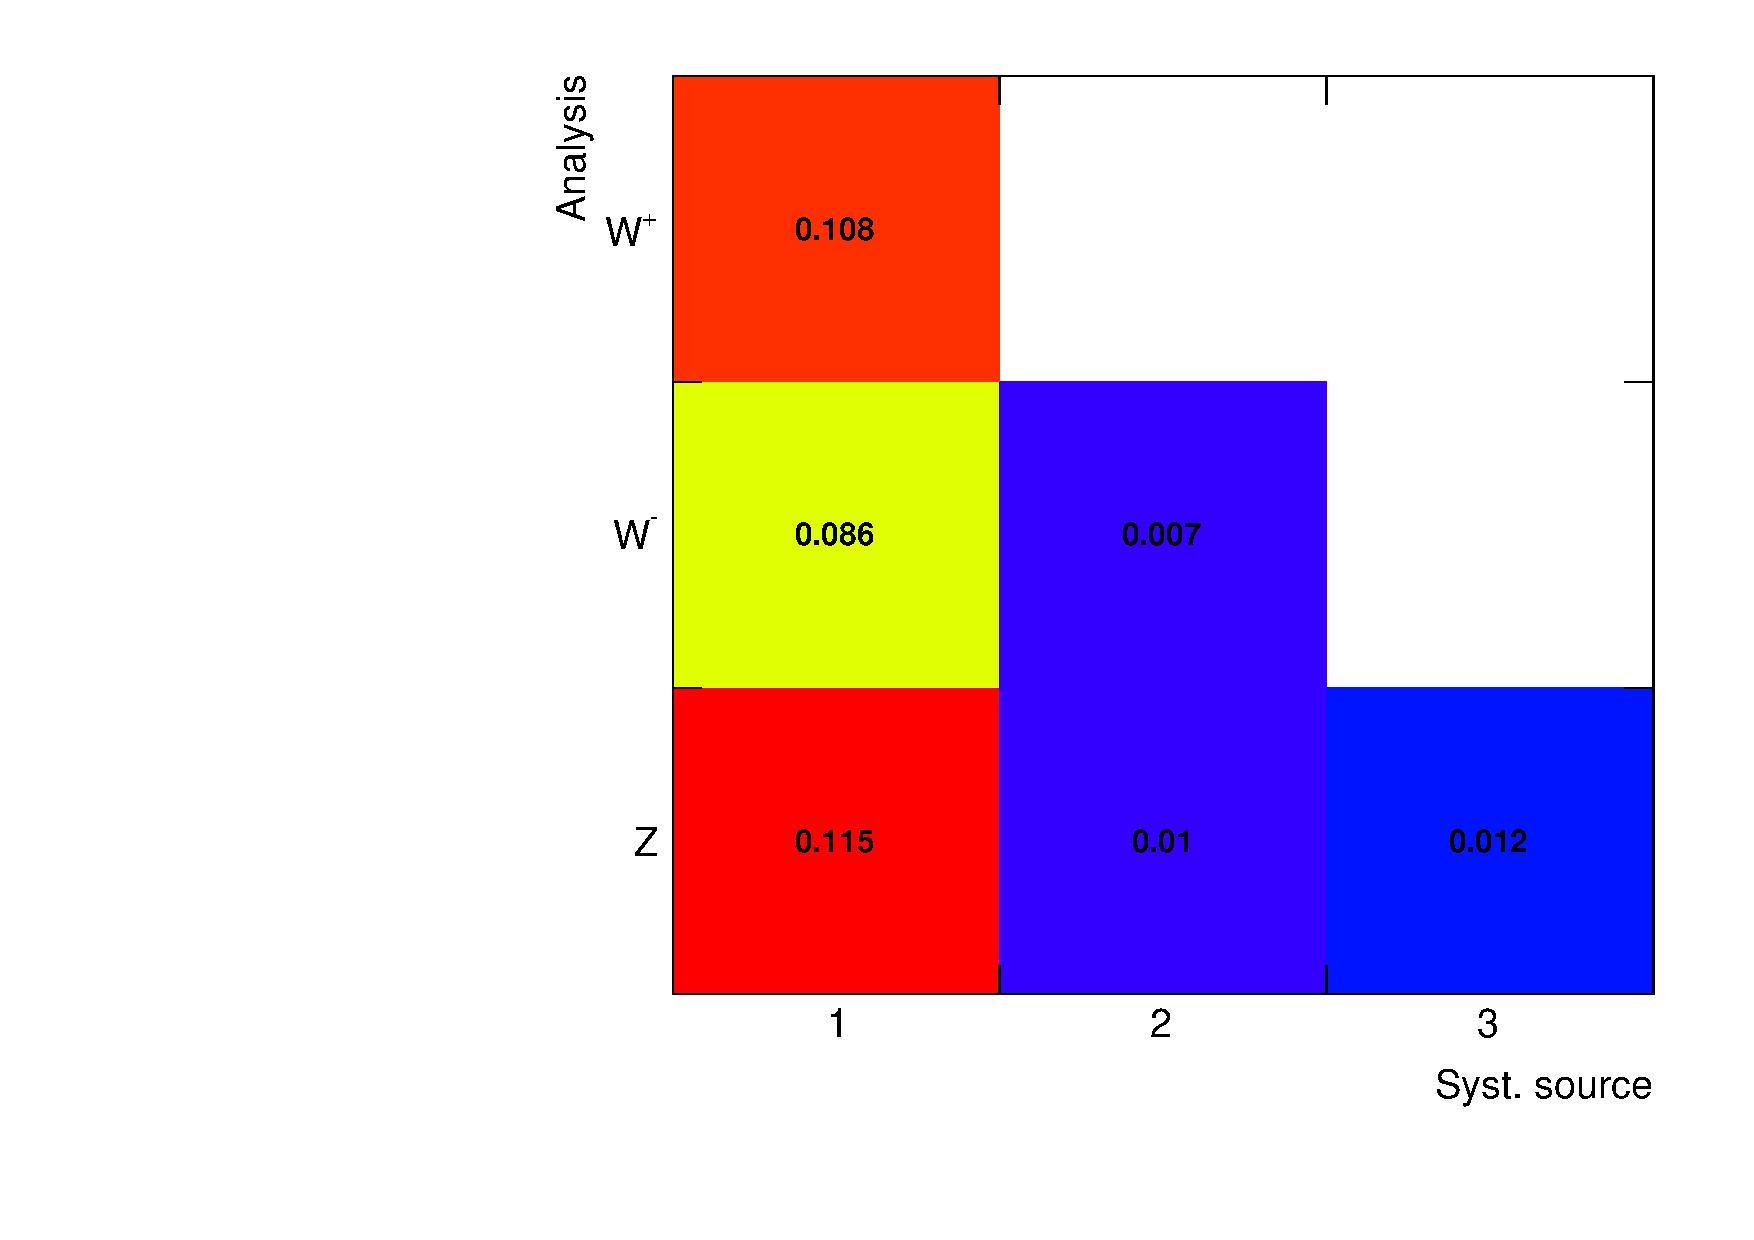
\includegraphics[width=1.0\linewidth]{Systematics/RecEffCl.pdf}  \\ a)}
\end{minipage}
\hfill
\begin{minipage}[h]{0.39\linewidth}
\center{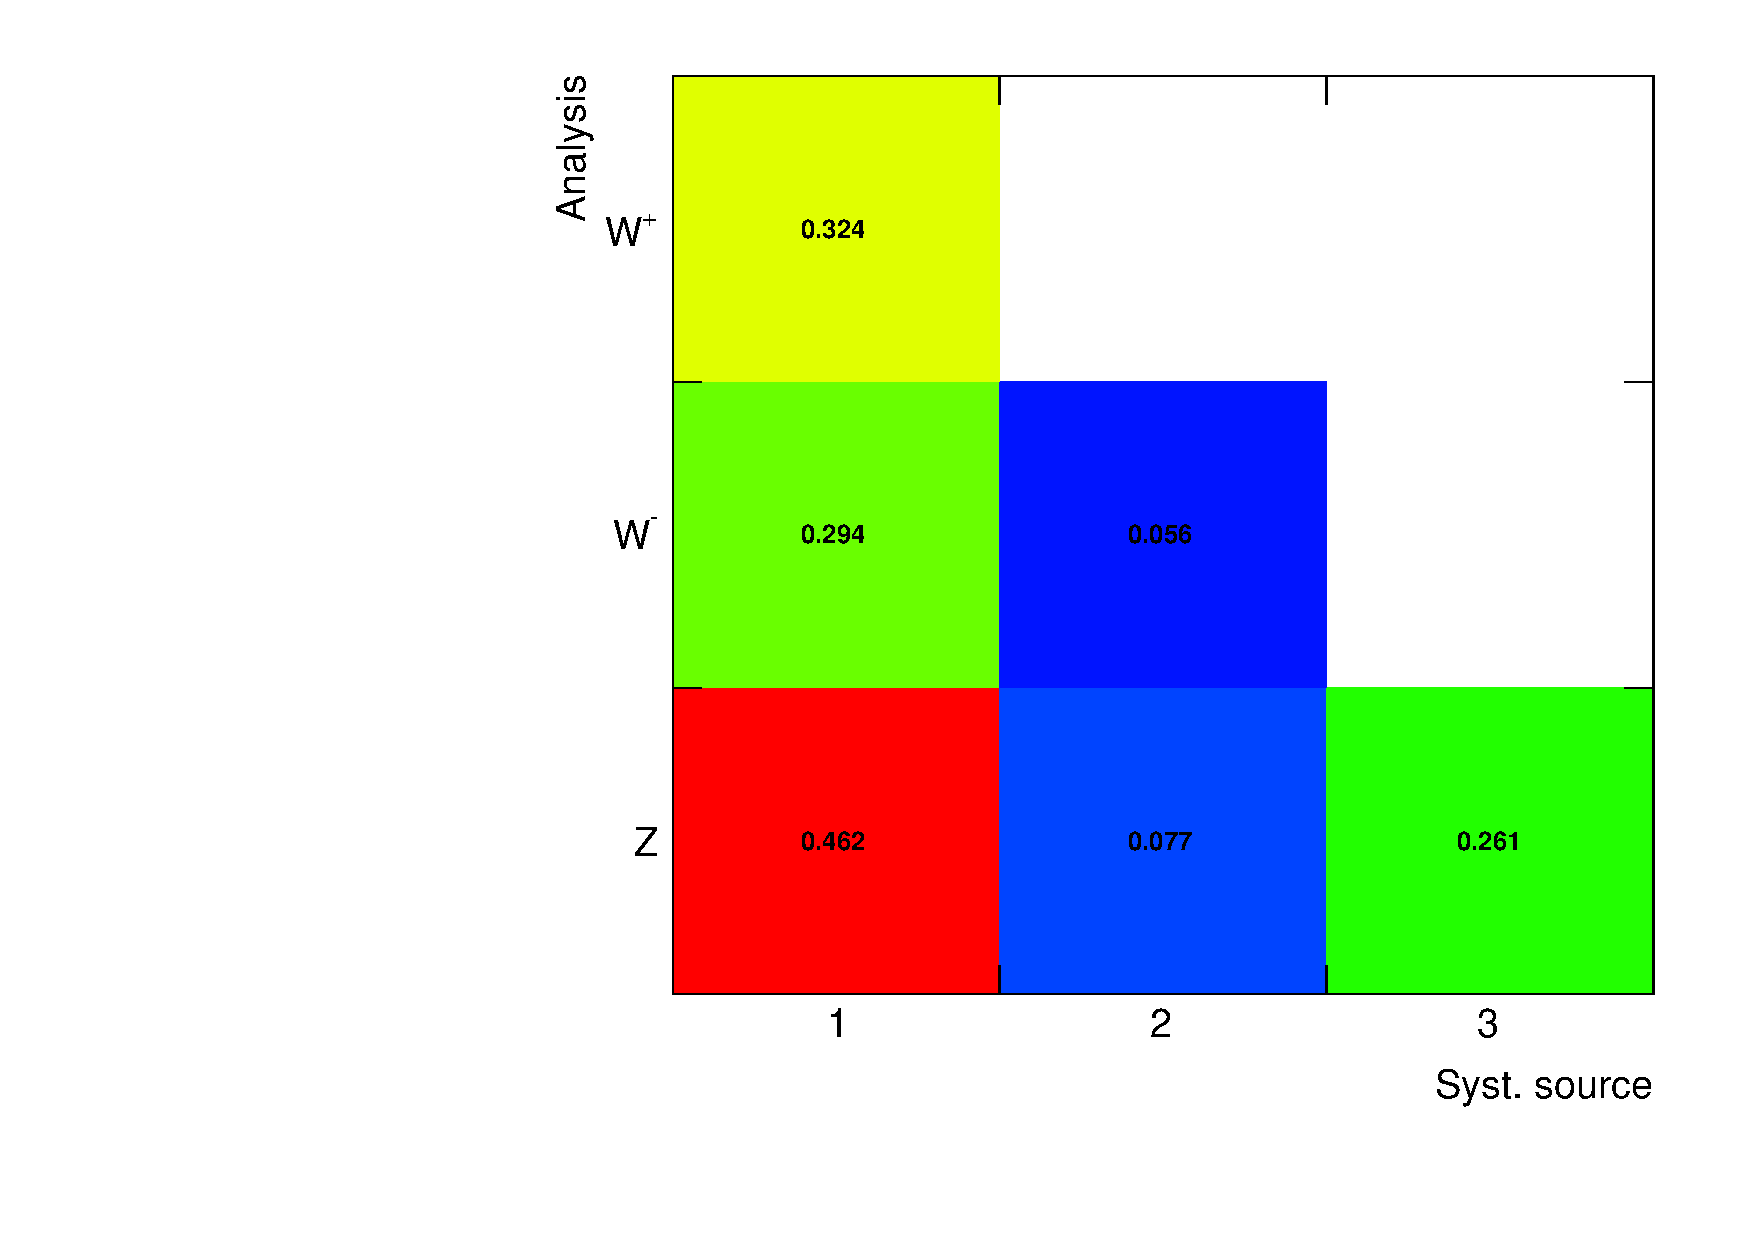
\includegraphics[width=1.0\linewidth]{Systematics/IDEffCl.pdf} \\ b)}
\end{minipage}
\vfill
\begin{minipage}[h]{0.39\linewidth}
\center{\includegraphics[width=1.0\linewidth]{Systematics/TrigCl.pdf}  \\ c)}
\end{minipage}
\hfill
\begin{minipage}[h]{0.39\linewidth}
\center{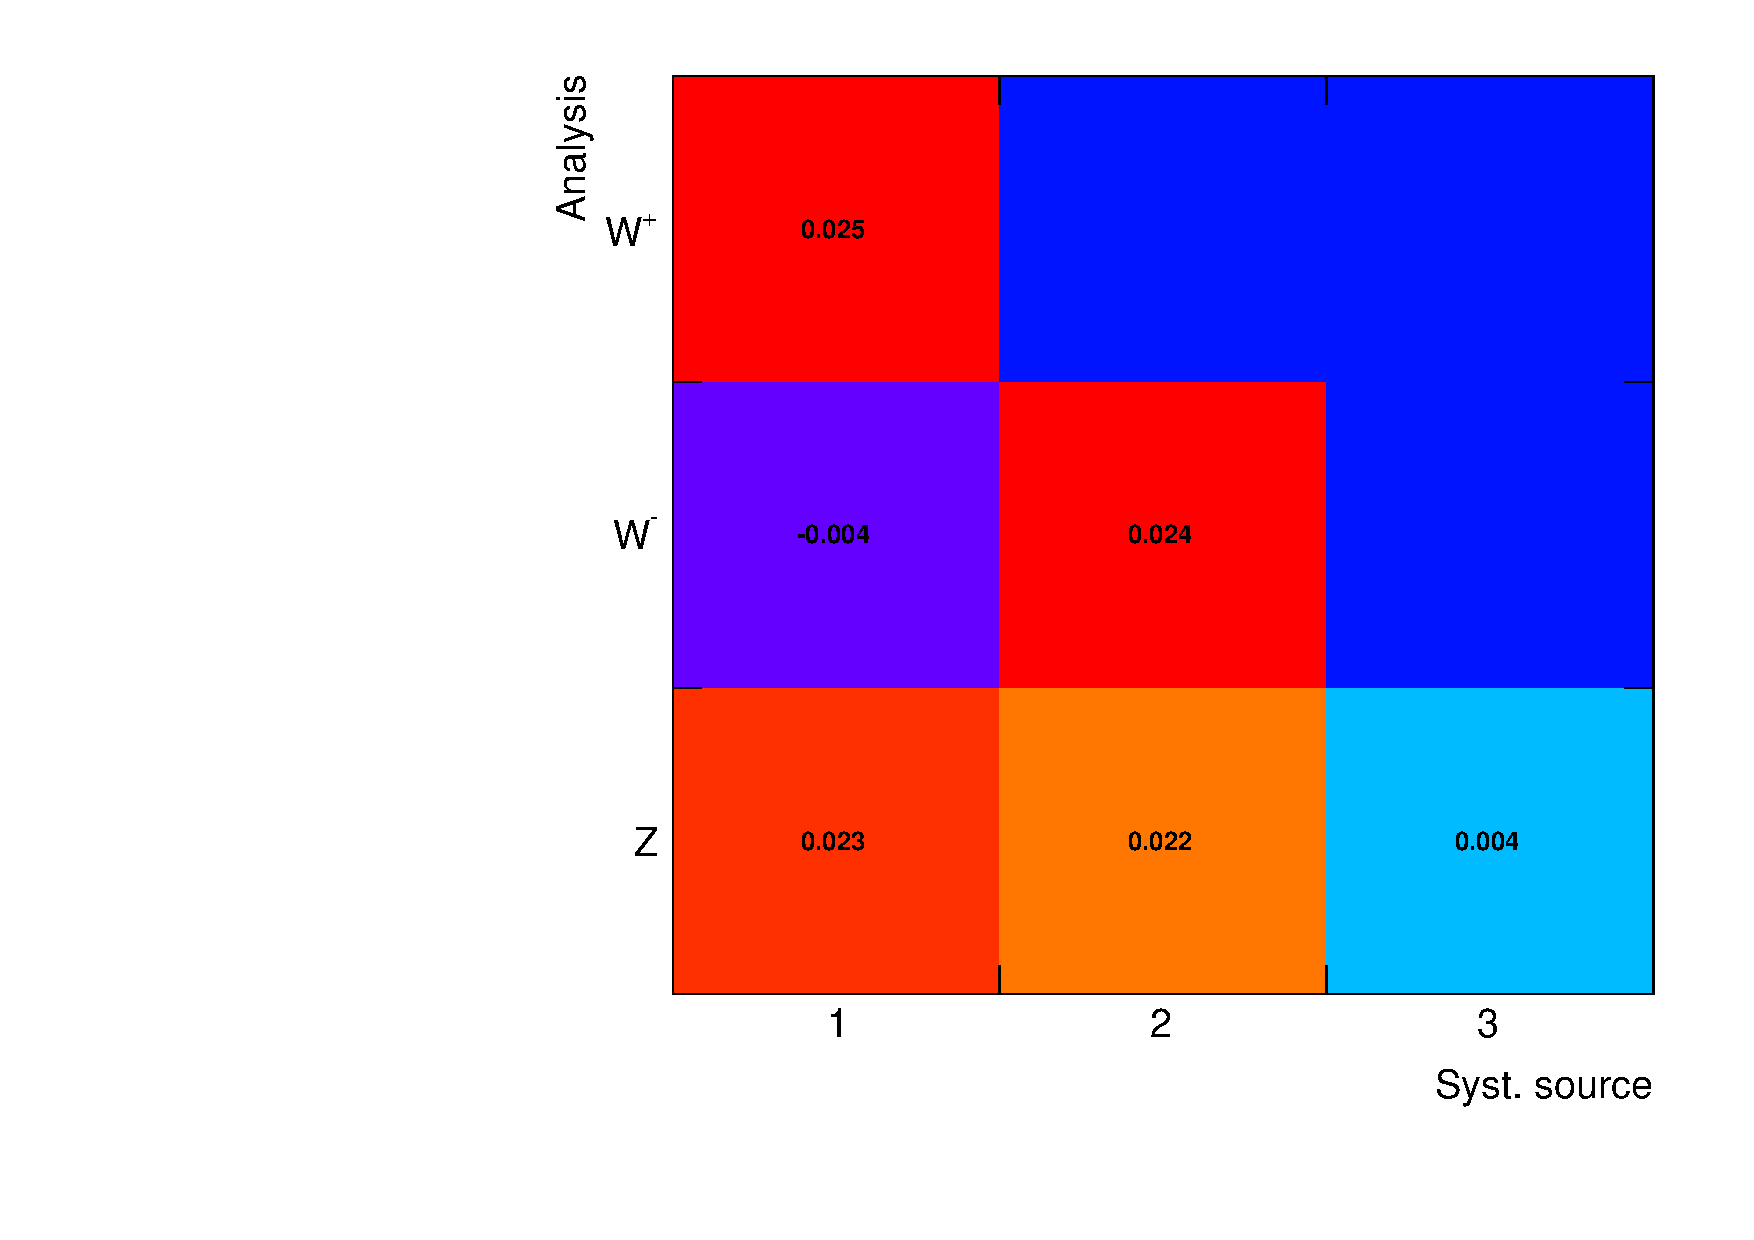
\includegraphics[width=1.0\linewidth]{Systematics/muIDEffCl.pdf} \\ d)}
\end{minipage}
\caption{Results of Cholesky decomposition for correlated uncertainties for a) electron reconstruction, b) electron identification, c) electron trigger and d) muon trigger scale factor uncertainties estimated using Toy MC method.}
\label{fig:AppA}
\end{figure}